\definecolor{zzttqq}{rgb}{0.15,0.35,0.15}

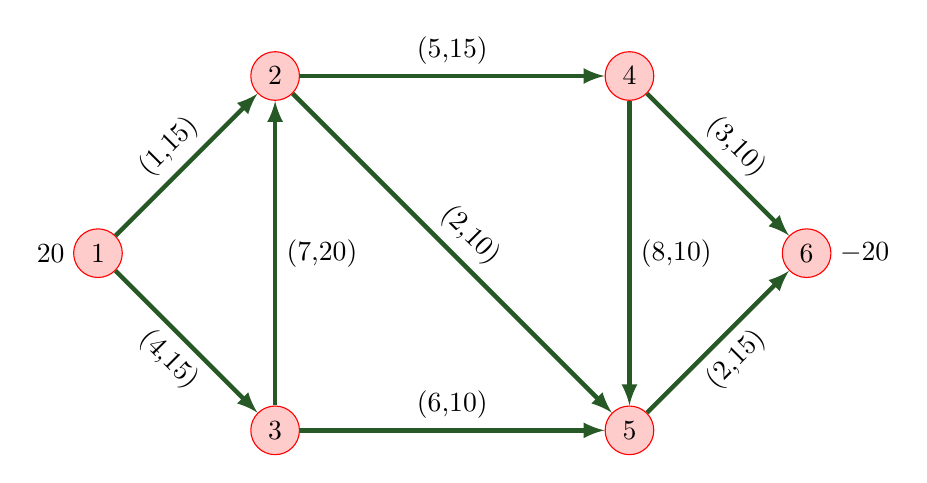
\begin{tikzpicture}[x=1.5cm, y=1.5cm]
	\fill (-3.2,0) circle (0.1pt)node[anchor=east] {$20$};
	\fill (3.2,0) circle (0.1pt)node[anchor=west] {$-20$};
    \node[circle,draw=red,fill=red!20!] (v2) at (-1.5,1.5) {2};
    \node[circle,draw=red,fill=red!20!] (v4) at (1.5,1.5) {4};
    \node[circle,draw=red,fill=red!20!] (v6) at (3,0) {6};
    \node[circle,draw=red,fill=red!20!] (v5) at (1.5,-1.5) {5};
    \node[circle,draw=red,fill=red!20!] (v3) at (-1.5,-1.5) {3};
    \node[circle,draw=red,fill=red!20] (v1) at (-3,0) {1};
    \draw[color=zzttqq, ultra thick, -latex]  (v1) edge node[rotate = 45, above,color=black]{(1,15)} (v2);
	\draw[color=zzttqq, ultra thick, -latex]  (v1) edge node[rotate = -45, below,color=black]{(4,15)} (v3);
	\draw[-latex, color=zzttqq, ultra thick]  (v3) edge node[right,color=black]{(7,20)} (v2);
	\draw[-latex, color=zzttqq, ultra thick]  (v2) edge node[above,color=black]{(5,15)} (v4);
	\draw[-latex, color=zzttqq, ultra thick]  (v3) edge node[above,color=black]{(6,10)} (v5);
	\draw[-latex, color=zzttqq, ultra thick]  (v2) edge node[rotate=-45,above,color=black]{(2,10)} (v5);
	\draw[-latex, color=zzttqq, ultra thick]  (v4) edge node[right,color=black]{(8,10)} (v5);
	\draw[-latex, color=zzttqq, ultra thick]  (v4) edge node[rotate=-45,above,color=black]{(3,10)} (v6);
	\draw[-latex, color=zzttqq, ultra thick]  (v5) edge node[rotate=45,below,color=black]{(2,15)} (v6);
    \end{tikzpicture}